% !TEX program = pdflatex
% -----------------------------------------------------------------------------
% MSc Dissertation Meeting Slides - Beamer template
% Easy-edit variables are grouped below. Compile from this directory with:
% pdflatex stock_forecasting_beamer.tex
% Optional generated assets can live in ../../outputs/.
% cnn_lstm_flow.pdf / gcn_layers_1_vs_2_summary.pdf when available.
% -----------------------------------------------------------------------------
\documentclass[aspectratio=169,11pt,t]{beamer}

\usetheme{default}
\usecolortheme{default}
\usefonttheme{professionalfonts}
\setbeamersize{text margin left=8mm,text margin right=8mm}
\setbeamertemplate{navigation symbols}{}
\setbeamertemplate{caption}[numbered]
\setbeameroption{hide notes} % change to show notes on second screen if needed

\usepackage[utf8]{inputenc}
\usepackage[utf8]{vietnam}
\usepackage{lmodern}
\usepackage{microtype}
\usepackage{amsmath,amssymb}
\usepackage{booktabs,array,multirow}
\usepackage{graphicx}
\usepackage{tikz}
\usetikzlibrary{arrows.meta,positioning,calc,fit,shapes.geometric}
\usepackage{xcolor}
\usepackage{tabularx}
\usepackage{ragged2e}

% -------------------------- Easy-edit project metadata ------------------------
\newcommand{\ProjectTitle}{Weekly Min-Max Stock Return Forecasting}
\newcommand{\ProjectSubtitle}{}

\newcommand{\StudentName}{Ha Hoang Hiep}
\newcommand{\PresentationDate}{28 June 2026}

% -------------------------- Easy-edit dataset values --------------------------
\newcommand{\NumStocks}{26}
\newcommand{\DateRange}{2019-06-28 to 2024-12-31}
\newcommand{\WeeklyPeriods}{288}
\newcommand{\WindowSize}{8}
\newcommand{\NumSequences}{280}
\newcommand{\NumFolds}{9}
\newcommand{\Seeds}{42, 52, 62}
\newcommand{\MainMetric}{$\mathrm{MAE}_{\mathrm{interval}} = \frac{1}{2}(\mathrm{MAE}_{min}+\mathrm{MAE}_{max})$}

% -------------------------- Academic presentation style -----------------------
\definecolor{paperbg}{HTML}{FAFAF8}
\definecolor{ink}{HTML}{111827}
\definecolor{muted}{HTML}{4B5563}
\definecolor{linegray}{HTML}{D7DCE2}
\definecolor{panelgray}{HTML}{F1F3F5}
\definecolor{deepblue}{HTML}{12355B}
\definecolor{researchteal}{HTML}{0E7490}
\definecolor{signalamber}{HTML}{B45309}
\definecolor{signalgreen}{HTML}{047857}
\definecolor{softblue}{HTML}{EAF1FF}
\definecolor{lightgray}{HTML}{F5F6F8}
\definecolor{darkgray}{HTML}{2D3748}
\definecolor{accentgreen}{HTML}{047857}
\definecolor{accentorange}{HTML}{B45309}
\colorlet{yorkblue}{deepblue}

\setbeamercolor{background canvas}{bg=paperbg}
\setbeamercolor{normal text}{fg=ink,bg=paperbg}
\setbeamercolor{title}{fg=deepblue}
\setbeamercolor{subtitle}{fg=muted}
\setbeamercolor{frametitle}{fg=deepblue,bg=paperbg}
\setbeamercolor{framesubtitle}{fg=muted}
\setbeamercolor{structure}{fg=deepblue}
\setbeamercolor{itemize item}{fg=researchteal}
\setbeamercolor{itemize subitem}{fg=researchteal}
\setbeamercolor{enumerate item}{fg=deepblue}
\setbeamercolor{block title}{bg=paperbg,fg=deepblue}
\setbeamercolor{block body}{bg=panelgray,fg=ink}
\setbeamercolor{alerted text}{fg=signalamber}
\setbeamercolor{headline}{bg=paperbg,fg=muted}
\setbeamercolor{footline}{bg=paperbg,fg=muted}
\setbeamercolor{keypointbox}{bg=deepblue!6,fg=ink}

\setbeamerfont{title}{series=\bfseries,size=\LARGE}
\setbeamerfont{subtitle}{size=\large}
\setbeamerfont{author}{size=\small}
\setbeamerfont{date}{size=\small}
\setbeamerfont{frametitle}{series=\bfseries,size=\Large}
\setbeamerfont{framesubtitle}{size=\small}
\setbeamerfont{block title}{series=\bfseries,size=\normalsize}
\setbeamerfont{block body}{size=\small}
\setbeamerfont{footline}{size=\scriptsize}
\setbeamerfont{headline}{size=\scriptsize}

\setbeamertemplate{itemize item}{\raise0.25ex\hbox{\tiny$\blacktriangleright$}}
\setbeamertemplate{itemize subitem}{\raise0.2ex\hbox{\tiny$\circ$}}
\setbeamertemplate{blocks}[default]
\setbeamertemplate{frametitle}{%
  \vspace{0.18cm}
  \begin{beamercolorbox}[wd=\paperwidth,leftskip=8mm,rightskip=8mm,sep=0pt]{frametitle}
    \usebeamerfont{frametitle}\insertframetitle\par
    {\usebeamerfont{framesubtitle}\usebeamercolor[fg]{framesubtitle}\insertframesubtitle}
  \end{beamercolorbox}
  \vspace{-0.03cm}
  \hspace{8mm}{\color{researchteal}\rule{18mm}{0.8pt}}{\color{linegray}\rule{\dimexpr\paperwidth-34mm\relax}{0.8pt}}
  \vspace{0.10cm}
}
\setbeamertemplate{headline}{}
\setbeamertemplate{footline}{%
  \ifnum\insertframenumber>1
  \begin{beamercolorbox}[wd=\paperwidth,ht=1.7ex,dp=0.6ex,leftskip=8mm,rightskip=8mm]{footline}
    \hfill\insertframenumber{} / \inserttotalframenumber 
  \end{beamercolorbox}
  \fi
}

\newcommand{\keypoint}[1]{%
  \begin{beamercolorbox}[wd=\textwidth,sep=4pt,leftskip=5pt,rightskip=5pt]{keypointbox}
    \footnotesize{} \justifying #1
  \end{beamercolorbox}
}
\newcommand{\smallcaps}[1]{\textsc{#1}}
\newcommand{\badge}[2]{%
  \tikz[baseline=(x.base)]\node[fill=#1,text=white,rounded corners=1pt,
  inner xsep=4pt,inner ysep=1.5pt,font=\scriptsize\bfseries](x){#2};}
\newcommand{\sectiontag}[1]{\badge{deepblue}{#1}}

\tikzset{
  box/.style={rounded corners=1pt, draw=deepblue, semithick, fill=deepblue!5, align=center, minimum height=0.78cm, inner sep=5pt},
  smallbox/.style={rounded corners=1pt, draw=linegray, fill=panelgray, align=center, minimum height=0.65cm, inner sep=4pt},
  arrow/.style={-{Latex[length=2.4mm]}, semithick, draw=muted},
  emphbox/.style={rounded corners=1pt, draw=signalgreen, semithick, fill=signalgreen!8, align=center, minimum height=0.75cm, inner sep=5pt}
}

\title[Weekly Min-Max Stock Return Forecasting]{\ProjectTitle}
\subtitle{\ProjectSubtitle}
\author[\StudentName]{\StudentName}
\date{\PresentationDate}

\begin{document}

% -----------------------------------------------------------------------------
\begin{frame}[plain]
  \begin{tikzpicture}[remember picture,overlay]
    \draw[linegray,line width=0.7pt] ([xshift=13mm,yshift=-15mm]current page.north west) -- ([xshift=-11mm,yshift=-15mm]current page.north east);
  \end{tikzpicture}
  \vspace*{1.15cm}
  \begin{center}
  \vspace{0.95cm}
  {\usebeamerfont{title}\usebeamercolor[fg]{title}\ProjectTitle\par}
  \vspace{0.48cm}
  \begin{tabular}{@{}ll@{}}
    \StudentName \\
    \PresentationDate \\
  \end{tabular}
  \vspace{1.0cm}
  \end{center}
  \note{Mở đầu bằng cách nói: phần trình bày này tóm tắt benchmark hiện tại, phát hiện chính, và research direction tiếp theo. Không bắt đầu bằng ``I built GAT-LSTM''. Bắt đầu từ bài toán forecasting.}
\end{frame}

% -----------------------------------------------------------------------------
\section{Tổng quan}
\begin{frame}{Outline}
\begin{block}{1. Experimental Setup}
\end{block}
\vspace{0.18cm}
\begin{block}{2. Empirical Results}
\end{block}
\vspace{0.18cm}
\begin{block}{3. Future Direction}
\end{block}

\end{frame}

% -----------------------------------------------------------------------------
\section{Problem setup}
\begin{frame}{Bài toán}
\begin{columns}[T,totalwidth=\textwidth]
\begin{column}{0.52\textwidth}
\begin{itemize}
  \item Forecast \textbf{min và max return tuần tiếp theo} cho từng stock.
  \item Input là \textbf{window dữ liệu 8 tuần} trên \NumStocks{} stocks.
  \item Có 4 baseline features: $f_{std}$, $f_{mean}$, $f_{return}$, $f_{skew}$.
\end{itemize}

\end{column}
\begin{column}{0.44\textwidth}
\centering
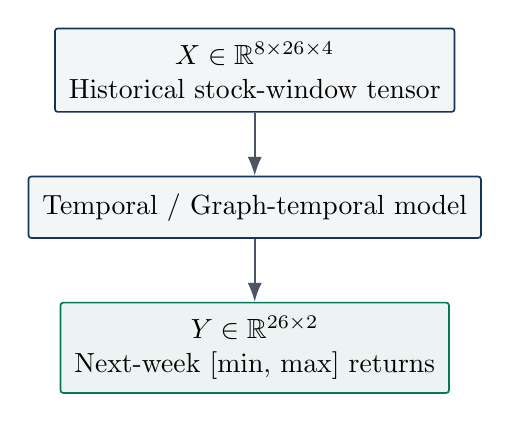
\begin{tikzpicture}[node distance=0.8cm]
  \node[box, minimum width=4.4cm] (x) {$X \in \mathbb{R}^{8 \times 26 \times 4}$\\Historical stock-window tensor};
  \node[box, below=of x, minimum width=4.4cm] (m) {Temporal / Graph-temporal model};
  \node[emphbox, below=of m, minimum width=4.4cm] (y) {$Y \in \mathbb{R}^{26 \times 2}$\\Next-week [min, max] returns};
  \draw[arrow] (x) -- (m);
  \draw[arrow] (m) -- (y);
\end{tikzpicture}
\end{column}
\end{columns}
\note{Nhấn mạnh X: [8, 26, 4] sang Y: [26, 2]. Điều này giúp bài toán cụ thể, không giống một stock forecasting project chung chung.}
\end{frame}

% -----------------------------------------------------------------------------
\section{Data và protocol}
\begin{frame}{Dataset và features}
\begin{columns}[T,totalwidth=\textwidth]
\begin{column}{0.48\textwidth}
\begin{block}{Data construction}
\begin{tabular}{@{}ll@{}}
\toprule
Stocks & \NumStocks{} \\
Daily price range & \DateRange{} \\
Aggregation & Daily $\rightarrow$ Weekly \\
Weekly periods & \WeeklyPeriods{} \\
Window size & \WindowSize{} weeks \\
Sequences & \NumSequences{} \\
\bottomrule
\end{tabular}
\end{block}
\end{column}
\begin{column}{0.48\textwidth}
\begin{block}{Feature set}
\begin{itemize}
  \item $f_{std}$: volatility
  \item $f_{mean}$: mean return 
  \item $f_{return}$: weekly return 
  \item $f_{skew}$: distribution asymmetry
\end{itemize}
\end{block}
\end{column}
\end{columns}

\note{Nói rằng additional indicators đã được test, nhưng final baseline giữ feature set ổn định. Tránh nói ``SMA12 is best'' vì full retuning không xác nhận điều đó.}
\end{frame}

% -----------------------------------------------------------------------------
\begin{frame}{Evaluation}
\begin{columns}[T,totalwidth=\textwidth]
\begin{column}{0.52\textwidth}
\begin{itemize}
  \item \textbf{Walk-forward expanding window} validation.
  \item \textbf{\NumFolds{} folds}
  % \item \textbf{27 runs cho mỗi model configuration}.
  \item Training loss: MSE.
  \item Evaluation metric: \MainMetric{}.
  \item Scaler chỉ fit trên training prefix.
\end{itemize}
\end{column}
\begin{column}{0.44\textwidth}
\centering
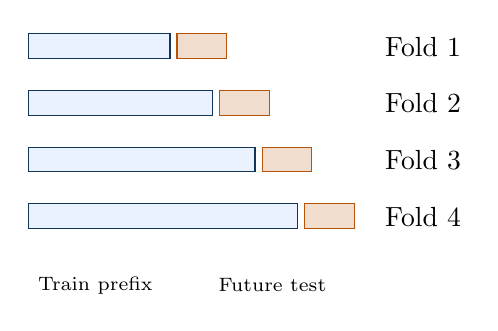
\begin{tikzpicture}[scale=0.9]
  \foreach \i/\w in {0/2.0,1/2.6,2/3.2,3/3.8} {
    \draw[fill=softblue, draw=yorkblue] (0,-\i*0.8) rectangle (\w,-\i*0.8-0.35);
    \draw[fill=accentorange!20, draw=accentorange] (\w+0.1,-\i*0.8) rectangle (\w+0.8,-\i*0.8-0.35);
    \node[anchor=west] at (4.9,-\i*0.8-0.18) {Fold \the\numexpr\i+1\relax};
  }
  \node[anchor=west] at (0,-3.55) {\scriptsize Train prefix};
  \node[anchor=west] at (2.55,-3.55) {\scriptsize Future test};
\end{tikzpicture}
\end{column}
\end{columns}
\vspace{0.1cm}

\note{Đây là methodological defence quan trọng. Nói rằng mỗi fold train trên quá khứ và test trên future period, giống deployment setting.}
\end{frame}

% -----------------------------------------------------------------------------
\section{Benchmark models}
\begin{frame}{Models}
\small
\begin{tabularx}{\textwidth}{@{}lX@{}}
\toprule
\textbf{Model} & \textbf{Ý tưởng chính} \\
\midrule
LSTM & Học pattern theo thời gian từ chuỗi 8 tuần của từng stock \\
GRU & Phiên bản RNN gọn hơn LSTM \\
CNN-LSTM & Dùng CNN tìm short-term local patterns \\
GCN-LSTM & Tổng hợp thông tin từ các stock hàng xóm trên graph cố định trước \\
GAT-LSTM & Học mức độ quan trọng của từng stock hàng xóm bằng attention trên graph \\
\bottomrule
\end{tabularx}

\note{Trình bày đây là một benchmark spectrum thống nhất, không phải 5 experiments rời rạc. Nhớ tí nói thì xóa phần Ý tưởng chính đi}
\end{frame}

% -----------------------------------------------------------------------------
\section{Kết quả}
\begin{frame}{Results}
\small
\centering
\begin{tabular}{@{}cllc@{}}
\toprule
\textbf{Rank} & \textbf{Model} & \textbf{Graph setting} & \textbf{MAE mean} \\
\midrule
1 & CNN-LSTM &  & \textbf{0.022189} \\
2 & GAT-LSTM & hybrid & 0.023120 \\
3 & LSTM &  & 0.023248 \\
4 & GAT-LSTM & static & 0.023650 \\
5 & GRU &  & 0.024032 \\
6 & GCN-LSTM & static & 0.024445 \\
7 & GCN-LSTM & hybrid & 0.026975 \\
\bottomrule
\end{tabular}

\note{Nói: CNN-LSTM hiện tốt nhất, GAT-LSTM khá gần, và graph models chưa consistently dominate temporal baselines. Dùng điều này làm motivation cho adaptive graph learning.}
\end{frame}

% -----------------------------------------------------------------------------
\section{Diễn giải}
\begin{frame}{CNN-LSTM}
\begin{columns}[T,totalwidth=\textwidth]
\begin{column}{0.48\textwidth}
\begin{itemize}
  \item CNN quét qua chuỗi 8 tuần của từng stock để tìm các pattern ngắn hạn.
  \item Max-pooling giữ lại những pattern nổi bật nhất và làm chuỗi đầu vào ngắn gọn hơn.
  \item LSTM sau đó học thứ tự xuất hiện của các pattern này để dự báo min và max return.
\end{itemize}

\end{column}
\begin{column}{0.48\textwidth}
\centering
\IfFileExists{../../outputs/cnn_lstm_flow.pdf}{
  \includegraphics[width=\textwidth,height=0.68\textheight,keepaspectratio]{../../outputs/cnn_lstm_flow.pdf}
}{
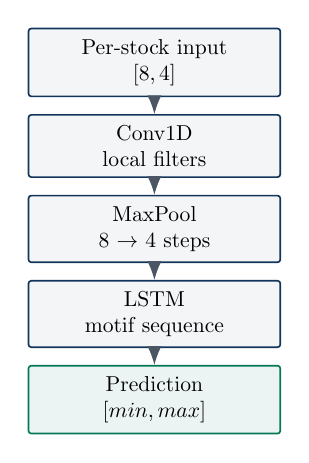
\begin{tikzpicture}[node distance=0.28cm, scale=0.78, transform shape]
  \node[box, minimum width=4.1cm, minimum height=0.58cm] (a) {Per-stock input\\$[8,4]$};
  \node[box, below=of a, minimum width=4.1cm, minimum height=0.58cm] (b) {Conv1D\\local filters};
  \node[box, below=of b, minimum width=4.1cm, minimum height=0.58cm] (c) {MaxPool\\8 $\rightarrow$ 4 steps};
  \node[box, below=of c, minimum width=4.1cm, minimum height=0.58cm] (d) {LSTM\\motif sequence};
  \node[emphbox, below=of d, minimum width=4.1cm, minimum height=0.58cm] (e) {Prediction\\$[min,max]$};
  \draw[arrow] (a)--(b); \draw[arrow] (b)--(c); \draw[arrow] (c)--(d); \draw[arrow] (d)--(e);
\end{tikzpicture}
}
\end{column}
\end{columns}
\note{Nếu asset SVG/PDF thật có sẵn, nó sẽ thay thế fallback TikZ diagram.}
\end{frame}

% -----------------------------------------------------------------------------
\begin{frame}{Graph models}
\begin{columns}[T,totalwidth=\textwidth]
\begin{column}{0.50\textwidth}
\begin{itemize}
  \item GCN phụ thuộc vào \textbf{predefined edges}.
  \item GAT học attention weights trên existing edges, \textbf{không} quyết định edges nào tồn tại.
  \item Hybrid graphs có thể thêm noise hoặc dense connections.
  \item Small sample size làm tăng overfitting risk cho graph models.
\end{itemize}

\end{column}
\begin{column}{0.46\textwidth}
\centering
\IfFileExists{../../outputs/gcn_layers_1_vs_2_summary.pdf}{
  \includegraphics[width=\textwidth,height=0.68\textheight,keepaspectratio]{../../outputs/gcn_layers_1_vs_2_summary.pdf}
}{
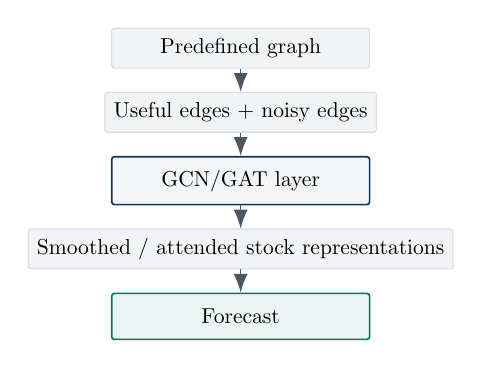
\begin{tikzpicture}[node distance=0.38cm, scale=0.78, transform shape]
  \node[smallbox, minimum width=4.2cm] (g) {Predefined graph};
  \node[smallbox, below=of g, minimum width=4.2cm] (edges) {Useful edges + noisy edges};
  \node[box, below=of edges, minimum width=4.2cm] (gat) {GCN/GAT layer};
  \node[smallbox, below=of gat, minimum width=4.2cm] (rep) {Smoothed / attended stock representations};
  \node[emphbox, below=of rep, minimum width=4.2cm] (pred) {Forecast};
  \draw[arrow] (g)--(edges);
  \draw[arrow] (edges)--(gat);
  \draw[arrow] (gat)--(rep);
  \draw[arrow] (rep)--(pred);
\end{tikzpicture}
}
\end{column}
\end{columns}
\note{Điểm quan trọng: GAT học attention trên supplied edges; điều này không giống học graph from scratch.}
\end{frame}

% -----------------------------------------------------------------------------
% \begin{frame}{Bài học từ feature engineering}
% \begin{columns}[T,totalwidth=\textwidth]
% \begin{column}{0.47\textwidth}
% \begin{block}{Đã test những gì}
% \begin{itemize}
%   \item Đã screen 60 technical feature variants.
%   \item SMA12 có vẻ promising trong single-feature sweep.
%   \item Sau full retuning, Baseline4 vẫn robust hơn.
% \end{itemize}
% \end{block}
% \end{column}
% \begin{column}{0.49\textwidth}
% \begin{block}{Diễn giải}
% \begin{itemize}
%   \item More features có thể làm giảm usable periods do rolling windows.
%   \item Indicator variants có thể redundant với existing return statistics.
%   \item Với small financial data, extra features có thể tăng noise và overfitting.
% \end{itemize}
% \end{block}
% \end{column}
% \end{columns}
% \vspace{0.2cm}
% \keypoint{Feature expansion không tự động có lợi; robustness sau full retuning quan trọng hơn một screening result đơn lẻ.}
% \note{Cẩn thận: không claim SMA12 là final selected feature. Nói nó là useful candidate nhưng không robust sau full retuning.}
% \end{frame}

% -----------------------------------------------------------------------------
\section{Research direction}
\begin{frame}{Research gap}
\begin{enumerate}
  \item Temporal models hoạt động tốt, nhưng không có mối quan hệ giữa các stock.
  \item GCN/GAT sử dụng quan hệ giữa các stocks, nhưng phụ thuộc vào chất lượng của predefined graphs.
  \item Transformer models có thể quá lớn với \NumSequences{} sequences và \NumStocks{} stocks.
\end{enumerate}
\vspace{0.35cm}
\begin{block}{Research question}
Một \textbf{lightweight adaptive graph-temporal model} có thể học được mối quan hệ ẩn và cải thiện kết quả trên tập dataset nhỏ không?
\end{block}
\note{Đây là chuyển tiếp quan trọng từ benchmark sang research contribution. Benchmark tạo ra research gap.}
\end{frame}

% % -----------------------------------------------------------------------------
% \begin{frame}{Đề xuất: Adaptive graph-temporal network}
% \centering
% \begin{tikzpicture}[node distance=0.48cm, scale=0.86, transform shape]
%   \node[box, minimum width=4.7cm, minimum height=0.62cm] (x) {$X \in \mathbb{R}^{B \times T \times N \times F}$\\8-week stock-feature tensor};
%   \node[box, below left=0.62cm and -0.2cm of x, minimum width=4.0cm, minimum height=0.62cm] (a) {Adaptive graph learning\\$A_{learned}=\mathrm{softmax}(E_1E_2^T)$};
%   \node[box, below right=0.62cm and -0.2cm of x, minimum width=4.0cm, minimum height=0.62cm] (t) {Light temporal module\\TCN / small attention};
%   \node[box, below=1.5cm of x, minimum width=4.9cm, minimum height=0.62cm] (f) {Graph-temporal fusion\\small hidden size, few layers};
%   \node[emphbox, below=of f, minimum width=4.6cm, minimum height=0.62cm] (y) {$\hat{Y} \in \mathbb{R}^{B \times N \times 2}$\\next-week min-max returns};
%   \draw[arrow] (x)--(a); \draw[arrow] (x)--(t);
%   \draw[arrow] (a)--(f); \draw[arrow] (t)--(f);
%   \draw[arrow] (f)--(y);
% \end{tikzpicture}
% \vspace{0.12cm}
% \keypoint{Contribution: so sánh adaptive stock relations với manually predefined graphs trong small financial data.}
% \note{Nói: Tôi không đề xuất full large Transformer. Hướng đi là small graph-temporal model với adaptive adjacency.}
% \end{frame}

% % -----------------------------------------------------------------------------
% \begin{frame}{Fair comparison plan cho lightweight model}
% \begin{columns}[T,totalwidth=\textwidth]
% \begin{column}{0.48\textwidth}
% \begin{block}{Giữ strong baselines}
% \begin{itemize}
%   \item LSTM, GRU
%   \item CNN-LSTM
%   \item GCN-LSTM, GAT-LSTM
% \end{itemize}
% \end{block}
% \end{column}
% \begin{column}{0.48\textwidth}
% \begin{block}{Thêm lightweight baselines}
% \begin{itemize}
%   \item DLinear / NLinear
%   \item TCN-lite
%   \item TSMixer-small
% \end{itemize}
% \end{block}
% \end{column}
% \end{columns}
% \vspace{0.25cm}
% \begin{block}{Cần report}
% Accuracy, parameter count, training time, inference time, và ablations: static graph vs hybrid graph vs adaptive graph.
% \end{block}
% \note{Slide này trả lời câu hỏi dự kiến từ supervisor: nếu proposed model là lightweight, cần so sánh với cả heavy strong baselines và lightweight baselines khác.}
% \end{frame}

% % -----------------------------------------------------------------------------
% \begin{frame}{Next experiments}
% \begin{enumerate}
%   \item Thêm TCN và DLinear/NLinear lightweight baselines.
%   \item Implement Adaptive Graph TCN-lite.
%   \item So sánh static, hybrid, và adaptive graph settings.
%   \item Chạy ablations: no graph, adaptive graph only, temporal module only, full model.
%   \item Interpret learned adjacency matrix theo sectors/correlation behaviour.
%   \item Report efficiency-accuracy trade-off, không chỉ MAE.
% \end{enumerate}
% \vspace{0.25cm}
% \keypoint{Success có thể là đạt gần accuracy của GAT-LSTM/CNN-LSTM với complexity thấp hơn nhiều và giải thích rõ hơn learned stock relations.}
% \note{Đây là action plan thực tế. Làm rõ rằng bước tiếp theo không phải chạy thêm random models, mà là test một hypothesis cụ thể.}
% \end{frame}

% % -----------------------------------------------------------------------------
% \begin{frame}{Kết luận}
% \begin{columns}[T,totalwidth=\textwidth]
% \begin{column}{0.31\textwidth}
% \begin{block}{Đã làm}
% \begin{itemize}
%   \item Leakage-safe walk-forward benchmark
%   \item Tuned temporal và graph-temporal models
%   \item Baseline4 feature setup
% \end{itemize}
% \end{block}
% \end{column}
% \begin{column}{0.31\textwidth}
% \begin{block}{Rút ra}
% \begin{itemize}
%   \item CNN-LSTM mạnh nhất quan sát được
%   \item Graph không tự động giúp tốt hơn
%   \item Feature expansion có rủi ro
% \end{itemize}
% \end{block}
% \end{column}
% \begin{column}{0.31\textwidth}
% \begin{block}{Tiếp theo}
% \begin{itemize}
%   \item Adaptive graph learning
%   \item Lightweight baselines
%   \item Ablation và interpretability
% \end{itemize}
% \end{block}
% \end{column}
% \end{columns}
% \vspace{0.35cm}
% \begin{center}
% \large \badge{accentorange}{Cần feedback}\\[0.15cm]
% \textbf{Adaptive graph-temporal model} vs \textbf{lightweight temporal model first}?
% \end{center}
% \note{Kết thúc bằng cách hỏi feedback về research framing, không chỉ implementation details.}
% \end{frame}

% % -----------------------------------------------------------------------------
% \appendix
% \section{Phụ lục}
% \begin{frame}[plain]
%   \begin{tikzpicture}[remember picture,overlay]
%     \fill[deepblue] (current page.north west) rectangle ([xshift=7mm]current page.south west);
%     \draw[researchteal,line width=1.1pt] ([xshift=7mm]current page.north west) -- ([xshift=7mm]current page.south west);
%   \end{tikzpicture}
%   \vspace{1.7cm}
%   {\Huge\bfseries Phụ lục\par}
%   \vspace{0.35cm}
%   {\large\color{muted} Backup answers cho technical discussion\par}
% \end{frame}

% % -----------------------------------------------------------------------------
% \begin{frame}{Backup: walk-forward folds}
% \small
% \begin{block}{Expanding-window evaluation}
% Mỗi fold train một fresh model trên available past và test trên future block tiếp theo.
% \end{block}
% \vspace{0.15cm}
% \centering
% \begin{tabular}{@{}cccc@{}}
% \toprule
% \textbf{Fold} & \textbf{Train samples} & \textbf{Test samples} & \textbf{Diễn giải} \\
% \midrule
% 1 & 0--150 & 150--165 & first future block \\
% 2 & 0--165 & 165--180 & train expands \\
% 3 & 0--180 & 180--195 & train expands \\
% $\cdots$ & $\cdots$ & $\cdots$ & $\cdots$ \\
% 9 & 0--270 & 270--280 & final future block \\
% \bottomrule
% \end{tabular}
% \vspace{0.3cm}
% \keypoint{Không fold nào train trên samples xảy ra sau test period của nó; đây là defence chính chống temporal leakage.}
% \end{frame}

% % -----------------------------------------------------------------------------
% \begin{frame}{Backup: so sánh graph settings}
% \small
% \begin{columns}[T,totalwidth=\textwidth]
% \begin{column}{0.31\textwidth}
% \begin{block}{Static graph}
% \begin{itemize}
%   \item Sector/domain prior
%   \item Cùng graph cho mọi windows
%   \item Stable nhưng có thể miss hidden relations
% \end{itemize}
% \end{block}
% \end{column}
% \begin{column}{0.31\textwidth}
% \begin{block}{Hybrid graph}
% \begin{itemize}
%   \item Static graph + dynamic edges
%   \item Dynamic edges từ within-window correlation
%   \item Flexible hơn nhưng có thể thêm noise
% \end{itemize}
% \end{block}
% \end{column}
% \begin{column}{0.31\textwidth}
% \begin{block}{Adaptive graph}
% \begin{itemize}
%   \item Learned dependency matrix
%   \item End-to-end stock relation learning
%   \item Proposed next direction
% \end{itemize}
% \end{block}
% \end{column}
% \end{columns}
% \vspace{0.2cm}
% \keypoint{Research question tiếp theo là liệu learned stock dependencies có hữu ích hơn manually predefined graph edges hay không.}
% \end{frame}

% % -----------------------------------------------------------------------------
% \begin{frame}{Backup: câu hỏi có thể gặp}
% \footnotesize
% \begin{tabularx}{\textwidth}{@{}p{0.32\textwidth}X@{}}
% \toprule
% \textbf{Câu hỏi} & \textbf{Trả lời} \\
% \midrule
% Vì sao không random split? & Financial series có time order. Random split có leakage risk; walk-forward chỉ test future blocks. \\
% \addlinespace[0.2ex]
% Vì sao CNN-LSTM thắng graph models? & Local temporal motifs có thể ổn định hơn noisy predefined graph edges trong small dataset này. \\
% \addlinespace[0.2ex]
% GAT có học graph không? & GAT học attention trên supplied edges. Nó không chọn edges nào tồn tại nếu graph không adaptive. \\
% \addlinespace[0.2ex]
% Vì sao không dùng full Transformer? & Với chỉ \NumSequences{} sequences, full Transformer dễ overfit. Lightweight design defensible hơn. \\
% \bottomrule
% \end{tabularx}
% \end{frame}

\end{document}
